
\subsection{JSynapse}

In order to test our protocols on real platforms, we have first
developed JSynapse, a Java-based software prototype, which uses Java
RMI standard for communications between nodes, and whose purpose is to
capture the very essence of our Synapse protocol. It is a flexible and
ready to be plugged library which can inter-connect any type of
overlay networks.  This prototype fully implements a Chord-based
inter-overlay network along with our original Maximum Replication Rate
mechanism. It is a lightweight easy to extend software. We also
provided some practical classes which help in automating the generation
of the inter-overlay network and the testing of specific scenarios.

We have experimented JSynapse on the Grid'5000 platform connecting
more than $20$ clusters on 9 different sites. Again, Chord was used as
the intra-overlay protocol.

In our first deployments, we used one cluster located at Sophia
Antipolis, France. The {\tt Helios} cluster is made of $56$ quad-core
AMD Opteron 275 linked by a gigabit Ethernet connection. The Synapse
network created was first made of up to $50$ processors uniformly
distributed among $3$ Chord intra-overlays. Then, still on the same
cluster, as nodes are quad-core, we deployed up to $3$ logical nodes
by processor, thus creating a $150$ nodes overlay network, nodes being
dispatched uniformly over $6$ overlays. During the deployment,
overlays were progressively bridged by synapses (whose
degree was always $2$).

Our goal is here to give a proof of concept and to show the viability
of the Synapse approach while confirming results obtained by
simulation. We also focused on the metrics affecting the user
(satisfaction ratio and time to get a response). In our deployment,
once his request was sent, a user waits only $1$ second before closing
channels opened to receive responses. If no response was received
after $1$ second, the query is considered as not satisfied.

Figure~\ref{dep:1-sat} shows the satisfaction ratio when increasing
the number of synapses. As expected, the general behavior is
comparable to the simulation results and a quasi-exhaustiveness is
achieved, with only a connectivity of $2$ for synapses.

\begin{figure}
        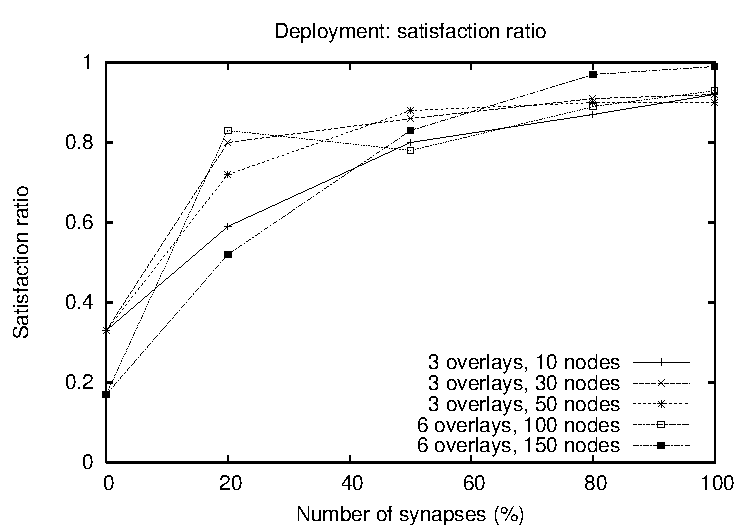
\includegraphics[width=\linewidth]{fig/dep1-sat.pdf}
        \caption{Deploying Synapse on the {\tt Helios} cluster -
        Exhaustiveness\label{dep:1-sat}}
\end{figure}

Figure~\ref{dep:1-time} illustrates the fact that, the latency
experienced by the user when launching a request is very low (few
milliseconds) even when a lot of synapses may generate a lot of
messages. Obviously this result has to be considered while keeping the
performances of the underlying hardware and network used in
mind. However, this suggests the viability of our protocols, the
confirmation of simulation results, and the efficiency of the software
developed.

\begin{figure}
        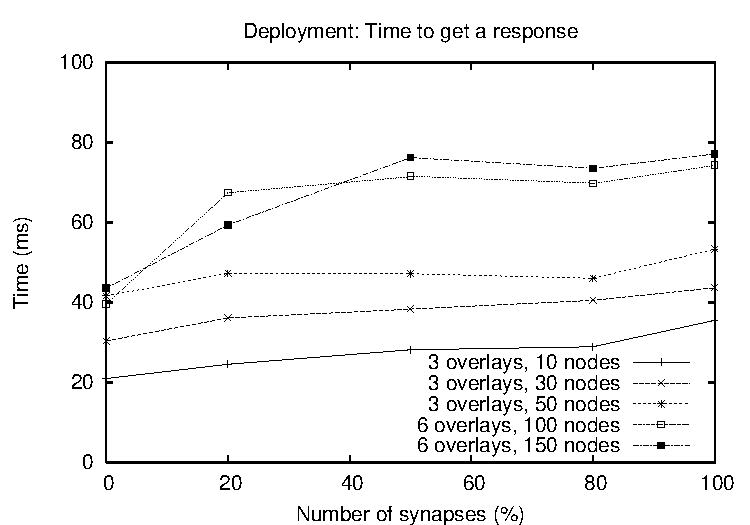
\includegraphics[width=\linewidth]{fig/dep1-time.pdf}
        \caption{Deploying Synapse on the {\tt Helios} cluster - Latency}
        \label{dep:1-time}
\end{figure}

\subsection{Open-Synapse}
%
We have also developed {\tt open-synapse}, based on the stable and
widely used {\tt open-chord} implementation, which provides a complete
and efficient Chord implementation. Open-Synapse has been developed as
an extension of the {\tt open-chord} core and thus takes advantage of
its robustness and reliability. A preliminary set of tests have been
successfully conducted on {\tt open-synapse}, involving $50$ nodes and
different randomly generated scenarii.
